% Generated by Sphinx.
\def\sphinxdocclass{report}
\documentclass[letterpaper,10pt,english]{sphinxmanual}
\usepackage[utf8]{inputenc}
\DeclareUnicodeCharacter{00A0}{\nobreakspace}
\usepackage[T1]{fontenc}
\usepackage{babel}
\usepackage{times}
\usepackage[Bjarne]{fncychap}
\usepackage{longtable}
\usepackage{sphinx}


\title{waveserv Documentation}
\date{June 15, 2012}
\release{devel}
\author{Brendan Smithyman}
\newcommand{\sphinxlogo}{}
\renewcommand{\releasename}{Release}
\makeindex

\makeatletter
\def\PYG@reset{\let\PYG@it=\relax \let\PYG@bf=\relax%
    \let\PYG@ul=\relax \let\PYG@tc=\relax%
    \let\PYG@bc=\relax \let\PYG@ff=\relax}
\def\PYG@tok#1{\csname PYG@tok@#1\endcsname}
\def\PYG@toks#1+{\ifx\relax#1\empty\else%
    \PYG@tok{#1}\expandafter\PYG@toks\fi}
\def\PYG@do#1{\PYG@bc{\PYG@tc{\PYG@ul{%
    \PYG@it{\PYG@bf{\PYG@ff{#1}}}}}}}
\def\PYG#1#2{\PYG@reset\PYG@toks#1+\relax+\PYG@do{#2}}

\def\PYG@tok@gd{\def\PYG@tc##1{\textcolor[rgb]{0.63,0.00,0.00}{##1}}}
\def\PYG@tok@gu{\let\PYG@bf=\textbf\def\PYG@tc##1{\textcolor[rgb]{0.50,0.00,0.50}{##1}}}
\def\PYG@tok@gt{\def\PYG@tc##1{\textcolor[rgb]{0.00,0.25,0.82}{##1}}}
\def\PYG@tok@gs{\let\PYG@bf=\textbf}
\def\PYG@tok@gr{\def\PYG@tc##1{\textcolor[rgb]{1.00,0.00,0.00}{##1}}}
\def\PYG@tok@cm{\let\PYG@it=\textit\def\PYG@tc##1{\textcolor[rgb]{0.25,0.50,0.56}{##1}}}
\def\PYG@tok@vg{\def\PYG@tc##1{\textcolor[rgb]{0.73,0.38,0.84}{##1}}}
\def\PYG@tok@m{\def\PYG@tc##1{\textcolor[rgb]{0.13,0.50,0.31}{##1}}}
\def\PYG@tok@mh{\def\PYG@tc##1{\textcolor[rgb]{0.13,0.50,0.31}{##1}}}
\def\PYG@tok@cs{\def\PYG@tc##1{\textcolor[rgb]{0.25,0.50,0.56}{##1}}\def\PYG@bc##1{\colorbox[rgb]{1.00,0.94,0.94}{##1}}}
\def\PYG@tok@ge{\let\PYG@it=\textit}
\def\PYG@tok@vc{\def\PYG@tc##1{\textcolor[rgb]{0.73,0.38,0.84}{##1}}}
\def\PYG@tok@il{\def\PYG@tc##1{\textcolor[rgb]{0.13,0.50,0.31}{##1}}}
\def\PYG@tok@go{\def\PYG@tc##1{\textcolor[rgb]{0.19,0.19,0.19}{##1}}}
\def\PYG@tok@cp{\def\PYG@tc##1{\textcolor[rgb]{0.00,0.44,0.13}{##1}}}
\def\PYG@tok@gi{\def\PYG@tc##1{\textcolor[rgb]{0.00,0.63,0.00}{##1}}}
\def\PYG@tok@gh{\let\PYG@bf=\textbf\def\PYG@tc##1{\textcolor[rgb]{0.00,0.00,0.50}{##1}}}
\def\PYG@tok@ni{\let\PYG@bf=\textbf\def\PYG@tc##1{\textcolor[rgb]{0.84,0.33,0.22}{##1}}}
\def\PYG@tok@nl{\let\PYG@bf=\textbf\def\PYG@tc##1{\textcolor[rgb]{0.00,0.13,0.44}{##1}}}
\def\PYG@tok@nn{\let\PYG@bf=\textbf\def\PYG@tc##1{\textcolor[rgb]{0.05,0.52,0.71}{##1}}}
\def\PYG@tok@no{\def\PYG@tc##1{\textcolor[rgb]{0.38,0.68,0.84}{##1}}}
\def\PYG@tok@na{\def\PYG@tc##1{\textcolor[rgb]{0.25,0.44,0.63}{##1}}}
\def\PYG@tok@nb{\def\PYG@tc##1{\textcolor[rgb]{0.00,0.44,0.13}{##1}}}
\def\PYG@tok@nc{\let\PYG@bf=\textbf\def\PYG@tc##1{\textcolor[rgb]{0.05,0.52,0.71}{##1}}}
\def\PYG@tok@nd{\let\PYG@bf=\textbf\def\PYG@tc##1{\textcolor[rgb]{0.33,0.33,0.33}{##1}}}
\def\PYG@tok@ne{\def\PYG@tc##1{\textcolor[rgb]{0.00,0.44,0.13}{##1}}}
\def\PYG@tok@nf{\def\PYG@tc##1{\textcolor[rgb]{0.02,0.16,0.49}{##1}}}
\def\PYG@tok@si{\let\PYG@it=\textit\def\PYG@tc##1{\textcolor[rgb]{0.44,0.63,0.82}{##1}}}
\def\PYG@tok@s2{\def\PYG@tc##1{\textcolor[rgb]{0.25,0.44,0.63}{##1}}}
\def\PYG@tok@vi{\def\PYG@tc##1{\textcolor[rgb]{0.73,0.38,0.84}{##1}}}
\def\PYG@tok@nt{\let\PYG@bf=\textbf\def\PYG@tc##1{\textcolor[rgb]{0.02,0.16,0.45}{##1}}}
\def\PYG@tok@nv{\def\PYG@tc##1{\textcolor[rgb]{0.73,0.38,0.84}{##1}}}
\def\PYG@tok@s1{\def\PYG@tc##1{\textcolor[rgb]{0.25,0.44,0.63}{##1}}}
\def\PYG@tok@gp{\let\PYG@bf=\textbf\def\PYG@tc##1{\textcolor[rgb]{0.78,0.36,0.04}{##1}}}
\def\PYG@tok@sh{\def\PYG@tc##1{\textcolor[rgb]{0.25,0.44,0.63}{##1}}}
\def\PYG@tok@ow{\let\PYG@bf=\textbf\def\PYG@tc##1{\textcolor[rgb]{0.00,0.44,0.13}{##1}}}
\def\PYG@tok@sx{\def\PYG@tc##1{\textcolor[rgb]{0.78,0.36,0.04}{##1}}}
\def\PYG@tok@bp{\def\PYG@tc##1{\textcolor[rgb]{0.00,0.44,0.13}{##1}}}
\def\PYG@tok@c1{\let\PYG@it=\textit\def\PYG@tc##1{\textcolor[rgb]{0.25,0.50,0.56}{##1}}}
\def\PYG@tok@kc{\let\PYG@bf=\textbf\def\PYG@tc##1{\textcolor[rgb]{0.00,0.44,0.13}{##1}}}
\def\PYG@tok@c{\let\PYG@it=\textit\def\PYG@tc##1{\textcolor[rgb]{0.25,0.50,0.56}{##1}}}
\def\PYG@tok@mf{\def\PYG@tc##1{\textcolor[rgb]{0.13,0.50,0.31}{##1}}}
\def\PYG@tok@err{\def\PYG@bc##1{\fcolorbox[rgb]{1.00,0.00,0.00}{1,1,1}{##1}}}
\def\PYG@tok@kd{\let\PYG@bf=\textbf\def\PYG@tc##1{\textcolor[rgb]{0.00,0.44,0.13}{##1}}}
\def\PYG@tok@ss{\def\PYG@tc##1{\textcolor[rgb]{0.32,0.47,0.09}{##1}}}
\def\PYG@tok@sr{\def\PYG@tc##1{\textcolor[rgb]{0.14,0.33,0.53}{##1}}}
\def\PYG@tok@mo{\def\PYG@tc##1{\textcolor[rgb]{0.13,0.50,0.31}{##1}}}
\def\PYG@tok@mi{\def\PYG@tc##1{\textcolor[rgb]{0.13,0.50,0.31}{##1}}}
\def\PYG@tok@kn{\let\PYG@bf=\textbf\def\PYG@tc##1{\textcolor[rgb]{0.00,0.44,0.13}{##1}}}
\def\PYG@tok@o{\def\PYG@tc##1{\textcolor[rgb]{0.40,0.40,0.40}{##1}}}
\def\PYG@tok@kr{\let\PYG@bf=\textbf\def\PYG@tc##1{\textcolor[rgb]{0.00,0.44,0.13}{##1}}}
\def\PYG@tok@s{\def\PYG@tc##1{\textcolor[rgb]{0.25,0.44,0.63}{##1}}}
\def\PYG@tok@kp{\def\PYG@tc##1{\textcolor[rgb]{0.00,0.44,0.13}{##1}}}
\def\PYG@tok@w{\def\PYG@tc##1{\textcolor[rgb]{0.73,0.73,0.73}{##1}}}
\def\PYG@tok@kt{\def\PYG@tc##1{\textcolor[rgb]{0.56,0.13,0.00}{##1}}}
\def\PYG@tok@sc{\def\PYG@tc##1{\textcolor[rgb]{0.25,0.44,0.63}{##1}}}
\def\PYG@tok@sb{\def\PYG@tc##1{\textcolor[rgb]{0.25,0.44,0.63}{##1}}}
\def\PYG@tok@k{\let\PYG@bf=\textbf\def\PYG@tc##1{\textcolor[rgb]{0.00,0.44,0.13}{##1}}}
\def\PYG@tok@se{\let\PYG@bf=\textbf\def\PYG@tc##1{\textcolor[rgb]{0.25,0.44,0.63}{##1}}}
\def\PYG@tok@sd{\let\PYG@it=\textit\def\PYG@tc##1{\textcolor[rgb]{0.25,0.44,0.63}{##1}}}

\def\PYGZbs{\char`\\}
\def\PYGZus{\char`\_}
\def\PYGZob{\char`\{}
\def\PYGZcb{\char`\}}
\def\PYGZca{\char`\^}
\def\PYGZsh{\char`\#}
\def\PYGZpc{\char`\%}
\def\PYGZdl{\char`\$}
\def\PYGZti{\char`\~}
% for compatibility with earlier versions
\def\PYGZat{@}
\def\PYGZlb{[}
\def\PYGZrb{]}
\makeatother

\begin{document}

\maketitle
\tableofcontents
\phantomsection\label{index::doc}


The \textbf{waveserv} program provides a web-based interface designed to simplify monitoring \href{http://orion.es.uwo.ca/index.php/FULLWV}{FULLWV} and \href{http://orion.es.uwo.ca/index.php/OMEGA}{OMEGA}.  It is specifically designed for use with this software, but is open-source and may be modified or reused freely.  While \textbf{waveserv} is less capable than a full seismic processing suite, it is compatible with a wide variety of devices and web browsers.  It also takes advantage of compression and advanced web techniques to make it very easy to monitor your server/cluster/workstation over a slow Internet connection.

The command-line program \textbf{waveserv} indexes all of the relevant files in the OMEGA/FULLWV project directory and provides them to the web browser of your choice.  This could (by default) be a browser on the same computer, or it could be a browser running on a computer half way around the world.  The interface is lightweight, and works fine on laptops, workstations, phones and tablets.  The server interface has been tested on Mac OS X and Linux, but will most likely work on any machine with a functional Python environment.  It is based on the development web server from the \href{http://www.djangoproject.com/}{Django Project}.

This package is licensed under the \href{http://www.opensource.org/licenses/BSD-3-Clause}{BSD License} (see project source for details).

The \textbf{waveserv} package also makes use of the \code{pygeo} Python module, and in particular the \code{pygeo.fullpy} interface for reading \emph{projnm.ini} files and \code{pygeo.segyread.SEGYFile} interface for reading the SEG-Y format datafiles used by OMEGA/FULLWV.  \code{pygeo} is released under the \href{http://www.opensource.org/licenses/lgpl-3.0.html}{GNU Lesser General Public License}.

Contents:


\chapter{Installation}
\label{installation:introduction}\label{installation:installation}\label{installation:intro}\label{installation::doc}\label{installation:id1}
\textbf{waveserv} can be accessed via \href{http://subversion.apache.org/}{Subversion} using the following command:

\begin{Verbatim}[commandchars=@\[\]]
svn co https://skylab.bitsmithy.net/svn/public/waveserv/trunk waveserv-base
\end{Verbatim}

This checks out the program source code into a directory called \textbf{waveserv-base}, using the SVN \emph{trunk} version.

\begin{notice}{note}{Note:}
The \emph{trunk} should always be (more or less) functional, but likely does not include the most up-to-date developments.  For the development version, issue:

\begin{Verbatim}[commandchars=@\[\]]
svn co https://skylab.bitsmithy.net/svn/public/waveserv/branches/devel waveserv-devel
\end{Verbatim}

However, note that the development version is not guaranteed to do anything other than possibly melt your computer; use at your own risk.
\end{notice}

In order to make \textbf{waveserv} available system-wide, you need to add the \textbf{waveserv-base} directory to the system search path.  For users of \textbf{bash} (Mac OS and Linux default in most cases), add the following to your \emph{\textasciitilde{}/.bash\_profile} or \emph{\textasciitilde{}/.bashrc} file:

\begin{Verbatim}[commandchars=@\[\]]
export PATH="/path/to/waveserv-base:@$PATH"
\end{Verbatim}

For users of \textbf{csh}, add the following to your \emph{\textasciitilde{}/.cshrc} file:

\begin{Verbatim}[commandchars=@\[\]]
setenv PATH "/path/to/waveserv-base:@$PATH"
\end{Verbatim}


\section{Custom Libraries}
\label{installation:custom-libraries}
\textbf{waveserv} requires the \code{pygeo} Python module in order to run.  To get a copy, issue the command:

\begin{Verbatim}[commandchars=@\[\]]
svn co https://skylab.bitsmithy.net/svn/public/pygeo/trunk pygeo-base
\end{Verbatim}

Place the directory \emph{pygeo-base} on your Python search path; in \textbf{bash}, this would look something like:

\begin{Verbatim}[commandchars=@\[\]]
if @PYGZlb[] -n "@$PYTHONPATH" @PYGZrb[]; then
  export PYTHONPATH="/path/to/pygeo-base:@$PYTHONPATH"
else
  export PYTHONPATH="/path/to/pygeo-base"
fi
\end{Verbatim}


\section{Generic Libraries}
\label{installation:generic-libraries}
This requires the following Python libraries installed on the system, and is tested with Python 2.6 or 2.7:

\begin{tabulary}{\linewidth}{|L|L|L|}
\hline
\textbf{
Package
} & \textbf{
Description
} & \textbf{
Minimum Version
}\\
\hline

python
 & 
Python Interpreter
 & 
Tested with 2.6+
\\

python-numpy
 & 
Numerical Python
 & 
Untested
\\

python-django
 & 
Django Web Framework
 & 
1.2
\\

python-matplotlib
 & 
Matlab-like plotting environment
 & 
Untested
\\
\hline
\end{tabulary}


If you are using Linux, I would expect all of the generic libraries to be in the package manager, but if not (e.g. CentOS has terrible Python support) they could be installed using another method like ``easy\_install''.  I have not tested with older versions of numpy and matplotlib, but I'm fairly sure that the Django framework needs to be at minimum v1.2.

\begin{notice}{note}{Note:}
If you are using Mac OS X (or if you want to use Python on MS Windows), I highly recommend the commercial \href{http://www.enthought.com/products/epd.php}{EPD (Enthought Python Distribution)}.  This is free for academic use, and reasonably priced for industry use given the level of support offered.  Additionally, there is a free version that most likely would suffice for casual use.  This can also be extremely handy for poorly-behaved Linux distributions.  Enthought supports Python development and open source.
\end{notice}


\chapter{Command Line Interface}
\label{cli:command-line-interface}\label{cli::doc}\label{cli:cli}
The \textbf{waveserv} CLI is a Python program that loads up a specially modified web server.  However, instead of hosting a web site, this interface looks for \href{http://orion.es.uwo.ca/index.php/Waveform\_Tomography}{Waveform Tomography} project files and generates an interactive listing.

You may run \textbf{waveserv} by navigating to the directory containing FULLWV/OMEGA files and typing \textbf{waveserv {[}projnm{]}}, where \textbf{{[}projnm{]}} is the name associated with the \textbf{*.ini} file.  It can also auto-detect this if there is only one project in the directory, but this fails (for example) during inversion because of the generation of \textbf{tmp.*} files.

Access the {\hyperref[gui:gui]{\emph{Graphical User Interface}}} by pointing a web browser at \href{http://localhost:1503/}{http://localhost:1503/} (by default), or use the command-line interface to change the port (``waveserv --help'').  If the server is not running on the local machine (i.e., your web browser is not on the machine that OMEGA/FULLWV runs on), you can specify the bind address as something other than \textbf{127.0.0.1}.  This is a potential security issue, so in most cases it is better to use VPN (Virtual Private Networking, e.g., \href{http://openvpn.net/}{OpenVPN}) or SSH-tunnel methods to access it from the local machine.  To set up a SSH tunnel, issue the following command on the machine running the web browser:

\begin{Verbatim}[commandchars=@\[\]]
ssh -f -N -L 1503:localhost:1503 @PYGZlb[]remotehost@PYGZrb[]
\end{Verbatim}

In this case, connect to the address \href{http://localhost:1503/}{http://localhost:1503/} as if you were running \textbf{waveserv} on the same computer.
\begin{figure}[htbp]
\centering
\capstart

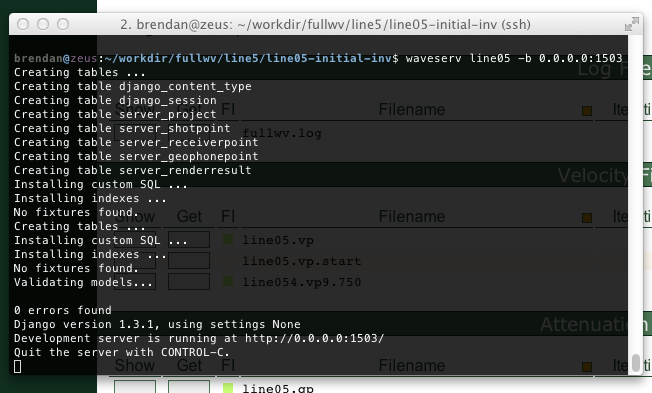
\includegraphics{startcmd9.png}
\caption{Example execution of \textbf{waveserv}, for a project named \emph{line05}.}\end{figure}

\begin{notice}{warning}{Warning:}
\textbf{waveserv} is based on the \href{http://www.djangoproject.com/}{Django} test web server.  This is designed for development use, and is not recommended for use on public networks (viz., the Internet).  \href{http://www.djangoproject.com/}{Django} is a popular project, and its vulnerabilities may be well-known; \textbf{waveserv} is susceptible to the same issues.  By default, \textbf{waveserv} is only accessible from the local computer, and so is only accessible to other users with accounts on the server/workstation.  The \emph{\texttt{-b}} option should only be used on a secure network.
\end{notice}


\section{Options}
\label{cli:options}
\indexii{waveserv command line option}{--version}

\begin{fulllineitems}
\phantomsection\label{cli:cmdoption-waveserv--version}\pysigline{\bfcode{--version}\code{}}{}\pysigline{\bfcode{show~program~version~number~and~exit}}{}
\end{fulllineitems}


\indexii{waveserv command line option}{-h, --help}

\begin{fulllineitems}
\phantomsection\label{cli:cmdoption-waveserv-h}\pysigline{\bfcode{-h}\code{}\code{,~}\bfcode{--help}\code{}}{}\pysigline{\bfcode{show~a~help~message~and~exit}}{}
\end{fulllineitems}


\indexii{waveserv command line option}{-v, --verbose}

\begin{fulllineitems}
\phantomsection\label{cli:cmdoption-waveserv-v}\pysigline{\bfcode{-v}\code{}\code{,~}\bfcode{--verbose}\code{}}{}\pysigline{\bfcode{display~additional~information}}{}
\end{fulllineitems}


\indexii{waveserv command line option}{-b ADDR, --bind=ADDR}

\begin{fulllineitems}
\phantomsection\label{cli:cmdoption-waveserv-b}\pysigline{\bfcode{-b}\code{~ADDR}\code{,~}\bfcode{--bind}\code{=ADDR}}{}\pysigline{\bfcode{server~address~to~bind~{[}Default:~127.0.0.1:1503{]}}}{}
\end{fulllineitems}


\indexii{waveserv command line option}{-d FILE, --db=FILE}

\begin{fulllineitems}
\phantomsection\label{cli:cmdoption-waveserv-d}\pysigline{\bfcode{-d}\code{~FILE}\code{,~}\bfcode{--db}\code{=FILE}}{}\pysigline{\bfcode{filename~for~server~database~{[}Default:~.waveserv.db{]}}}{}
\end{fulllineitems}


\indexii{waveserv command line option}{-g, --serverdebug}

\begin{fulllineitems}
\phantomsection\label{cli:cmdoption-waveserv-g}\pysigline{\bfcode{-g}\code{}\code{,~}\bfcode{--serverdebug}\code{}}{}\pysigline{\bfcode{enable~debugging~for~web~server}}{}
\end{fulllineitems}


\indexii{waveserv command line option}{-k, --keep}

\begin{fulllineitems}
\phantomsection\label{cli:cmdoption-waveserv-k}\pysigline{\bfcode{-k}\code{}\code{,~}\bfcode{--keep}\code{}}{}\pysigline{\bfcode{keep~temporary~files~on~exit~{[}Default:~False{]}}}{}
\end{fulllineitems}


\indexii{waveserv command line option}{-p DIBUPATH, --dibupath=DIBUPATH}

\begin{fulllineitems}
\phantomsection\label{cli:cmdoption-waveserv-p}\pysigline{\bfcode{-p}\code{~DIBUPATH}\code{,~}\bfcode{--dibupath}\code{=DIBUPATH}}{}\pysigline{\bfcode{path~for~temporary~image~files~{[}Default:~.buffer{]}}}{}
\end{fulllineitems}



\chapter{Graphical User Interface}
\label{gui:gui}\label{gui::doc}\label{gui:graphical-user-interface}
The \textbf{waveserv} program directly indexes and reads the (SEG-Y) files in the directory working directory on the server, handling endian and floating point conversion, and provides a directory listing through the web-browser interface.  The web-based GUI is rendered by the \textbf{waveserv} executable, which is started using a {\hyperref[cli:cli]{\emph{Command Line Interface}}}.

With the \textbf{waveserv} server running, navigate to \href{http://localhost:1503/index}{http://localhost:1503/index} to show the directory listing:
\begin{figure}[htbp]
\centering
\capstart

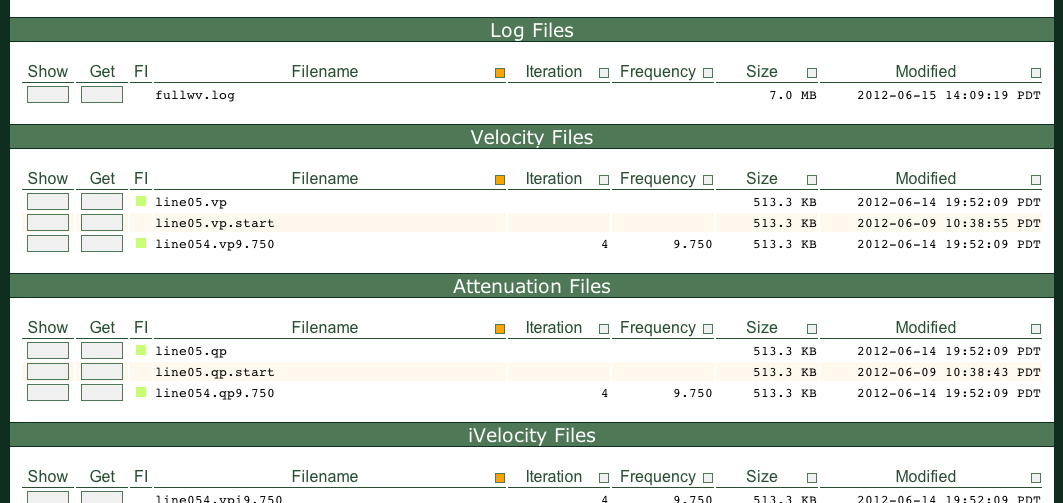
\includegraphics{listing4.png}
\caption{Directory listing rendered by \textbf{waveserv}.}\end{figure}

Each type of file is grouped under a descriptive heading, and the entries under each heading are sorted.  Several pieces of information are available for each entry, including the \emph{filename}, \emph{size}, and \emph{modification time}.  Additionally, for files that correspond to a particular \emph{frequency} or \emph{iteration}, this information is extracted from the filename.  Each of these headings can be used as a sort key; simply click the corresponding check box (beside the column heading) to change the sort key.  The current sort key is indicated by a box that is coloured differently from the others.
New in version 1.1: An indicator shows the freshness of each file graphically.
Each entry has two buttons, labelled \emph{Show} and \emph{Get}.  Clicking the \emph{Get} button simply downloads the original file.  The \emph{Show} button beside an entry displays a graphical representation of the file.  This takes you to \href{http://localhost:1503/show/filename}{http://localhost:1503/show/filename} for a file \emph{filename}, which is a web address that calls a plotting method, which generates a PNG image.
\begin{figure}[htbp]
\centering
\capstart

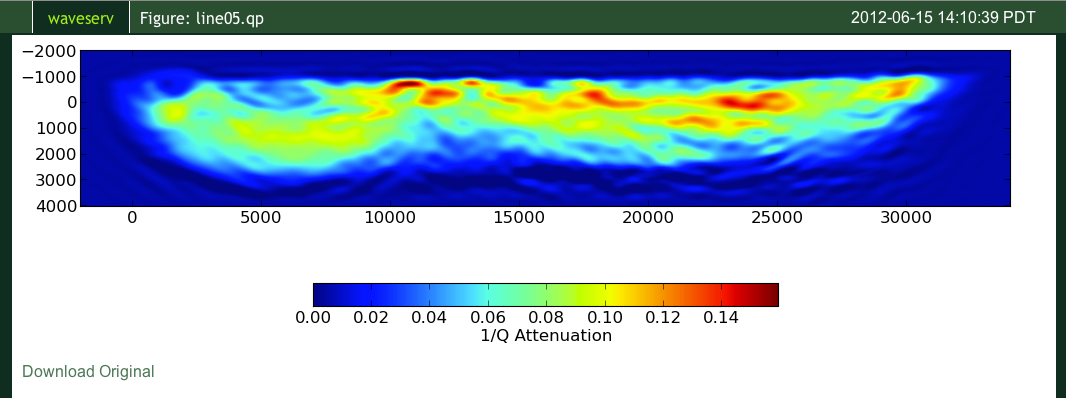
\includegraphics{qpmodel1.png}
\caption{Example plot for an attenuation (1/Q) model, for the project \emph{line05}.}\end{figure}


\chapter{Development}
\label{development:development}\label{development::doc}\label{development:devel}
To date, all development of \textbf{waveserv} has been by me alone (Brendan Smithyman).  I'd be more than pleased to have someone else interested in the development, so please feel free to send questions, comments or fixes to me at \href{mailto:bsmithyman@eos.ubc.ca}{bsmithyman@eos.ubc.ca}.


\section{Main Executable}
\label{development:main-executable}
The \textbf{waveserv} executable is written in Python, and uses \href{http://docs.python.org/library/optparse.html\#optparse}{\code{optparse}} to generate the {\hyperref[cli:cli]{\emph{Command Line Interface}}}.  It also creates a minimal database for the \code{django} test web server on the fly, using a temporary \href{http://docs.python.org/library/sqlite3.html\#sqlite3}{\code{sqlite3}} database to store the settings and data.  It imports the \code{django.core.management} interface, and uses this to construct a new \code{django} project in the working directory.  The \code{pygeo.fullpy} module is used to access the \textbf{projnm.ini} file from the working directory, and read the information.  This is stored in the \code{django} database.  While the current version of the interface does not implement this, there are provisions for storing source and receiver information, which would make it possible to plot sources and receivers over model images (or to create maps and geometry plots).

The vast majority of the web-server code is handled by the \code{django} test web server, which is called using the \code{django.core.management} interface near the end of the \textbf{waveserv} source.  Unless otherwise specified, temporary files are deleted at the end of the execution.


\section{Server Code}
\label{development:server-code}
The main logic of the \textbf{waveserv} program is managed by the server-side code in the \textbf{server/} directory:
\begin{description}
\item[{\textbf{urls.py}}] \leavevmode
This file determines the URL (Uniform Resource Locator) structure of the web-based interface.  This determines which Python function handles each URL (e.g., /index, /show/..., /download/...).

\item[{\textbf{models.py}}] \leavevmode
This file defines the database model for \textbf{waveserv}, which is necessary for storing information about the project (i.e., from the \textbf{projnm.ini} file).  The database is also used to store information for caching images; if the PNG image for a given geophysical datafile is more up-to-date than the file itself, a cached version is used rather than re-generating the figure.

\item[{\textbf{views.py}}] \leavevmode
This file contains code that deals with most/all of the \emph{web-server} aspects of \textbf{waveserv}.  This includes data processing for the listing page, the actual \emph{rendering} of figures, handling downloads, caching, etc.  The intent is for this to include most of the processing that is web-interface specific, and as such it makes heavy use of \code{django} design techniques.  With the exception of some initial data management code, this file is made up of a series of \emph{views}, which handle the server-side processing for web addresses listed in \textbf{urls.py}.

\item[{\textbf{handlers.py}}] \leavevmode
This file contains code that deals with most/all of the \emph{geophysical} aspects of \textbf{waveserv}.  This includes processing files, interfacing with geophysical data formats (viz., SEG-Y), generating figures in an abstract sense, and filesystem actions.  The file management is heavily dependent on the \href{http://docs.python.org/library/re.html\#re}{\code{re}} module (for \emph{regular expression} parsing); \textbf{waveserv} knows how to handle a particular file type because of the lookup tables in this source file.  In principle, this could be used to generate plots separately from the web interface (e.g., for scripted generation of figures in conjunction with document preparation).

\item[{\textbf{settings.py}}] \leavevmode
This file is not actually used by \textbf{waveserv} at all, but is required if you wish to test code using the regular \code{django} test server.

\item[{\textbf{manage.py}}] \leavevmode
This file is not actually used by \textbf{waveserv} at all, but is required if you wish to test code using the regular \code{django} test server.

\end{description}


\section{Media and Templates}
\label{development:media-and-templates}
The web interface is built using the \code{django} templating language, saved in a series of \textbf{*.html} files in the \textbf{templates/} directory.  These control most of the structural aspects of the GUI, and are populated with data using server-side Python scripting.  The visual elements are controlled mainly by a stylesheet stored in the \textbf{media/} directory.


\chapter{Indices and tables}
\label{index:indices-and-tables}\begin{itemize}
\item {} 
\emph{genindex}

\item {} 
\emph{modindex}

\item {} 
\emph{search}

\end{itemize}



\renewcommand{\indexname}{Index}
\printindex
\end{document}
